\chapter{Informatisation des infrastructures}

L'idée des Smart City et de l'informatisation de la gestion des villes n'est pas nouvelle.
Il y a eu beaucoup d'idées du type Science-Fiction dans les années 1800 qui pensaient la ville
complètement automatisée par des tubes, des trottoirs roulants, une gestion des déchets automatique.
Cette Science-Fiction a mis presque 150 ans à voir le jour.

\begin{figure}[h]
  \centering
  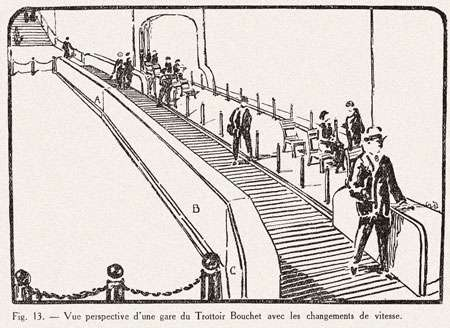
\includegraphics[scale=0.30]{media/trottoir_roulant.jpg}
  \caption{Trottoir roulant - Paris 1900 - Exposition Universelle}
\end{figure}

\section{Étude de Cybersyn}

Dans les années 1970 au Chili, Salvador Allende gagne les élections présidentielles.
En pleine guerre froide, le Chili devenu Socialiste se déclare neutre et n'est donc
contraint ni par les États-Unis, ni par l'URSS.

Le Chili a vu dans les années précédentes d'importantes famines. Le gouvernement voulait
absolument éviter ça. Malheureusement, de par la politique socialiste de l'époque,
tout était rationné et toutes les décisions sont prises d'en haut.
Pour éviter de finir comme l'URSS, qui a connu d'importantes famines dues a une
bureaucratie écrasante, l'État demanda à Fernando Flores de trouver une solution.

Fernando Flores est un ingénieur, entrepreneur et politicien chilien qui eu l'idée
d'automatiser le pays : tout ce qui permet d'aller vite évite la rétention d'information,
ainsi que des ralentissements inutiles pour l'avenir du pays.
Il décida d'inviter Stafford Beer pour s'occuper d'un tout nouveau projet d'une grande ampleur,
le projet Cybernet pour Cybernetic Synergy.

L'idée de base est simple. Obtenir en temps réel (c'est-à-dire une fois par jour pour l'époque)
l'état économique du pays pour aider à la prise de décisions.
Pour ce faire, chaque entité connectée au réseau devait envoyer un compte-rendu quotidien sur
la production de celle-ci. Ce compte-rendu est envoyé au niveau supérieur et est mis en commun
avec les autres entités.

\begin{figure}[h!]
  \centering
  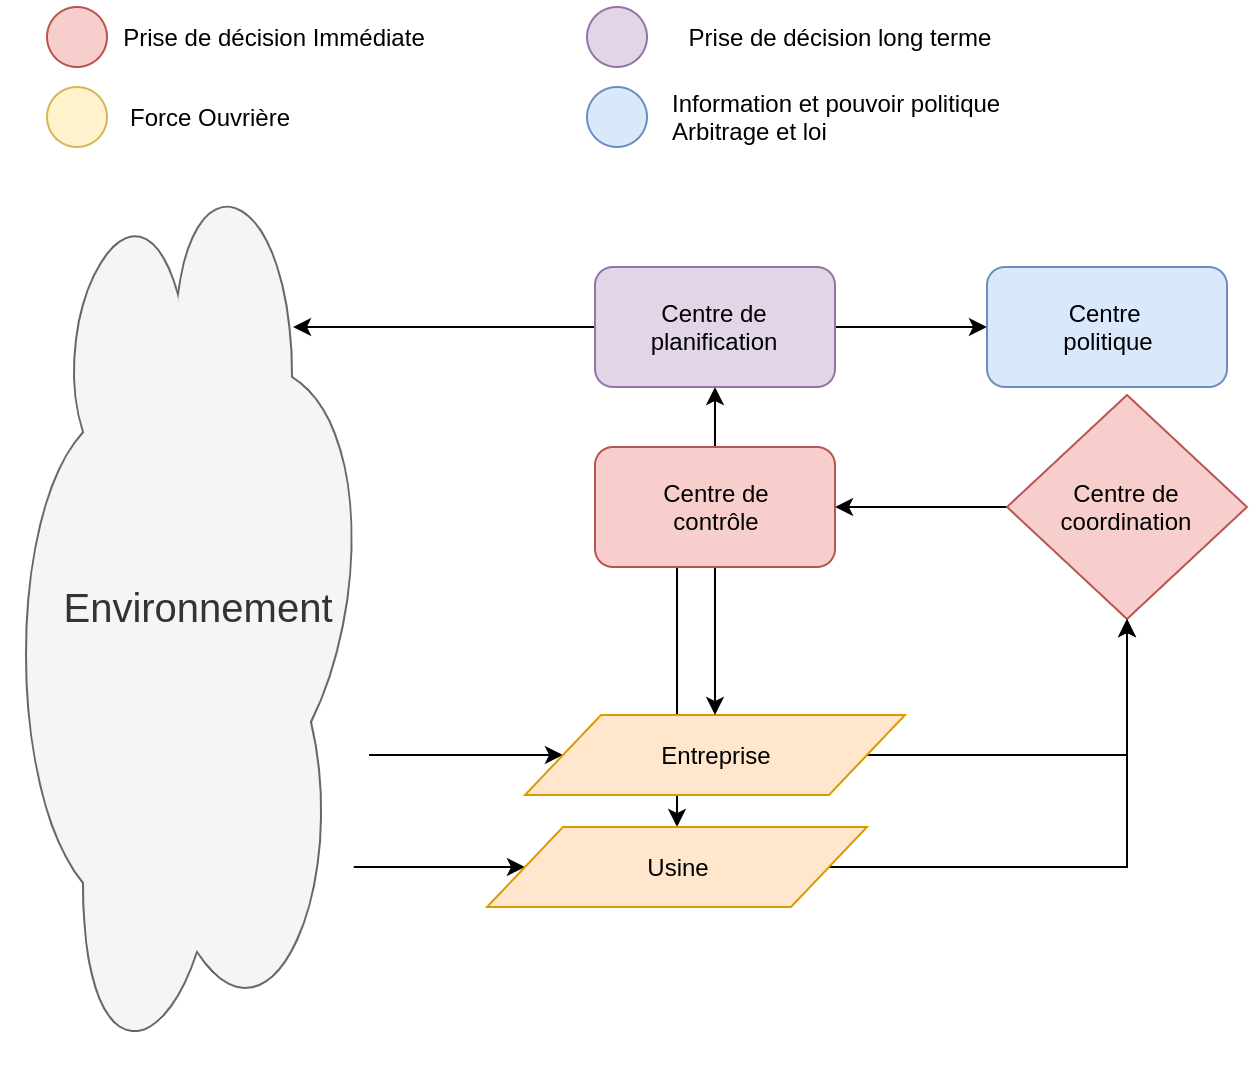
\includegraphics[scale=0.20]{media/cybersyn.png}
  \caption{Architecture du projet CyberSyn}
\end{figure}

Le projet était bien huilé. Les travailleurs remontaient les informations
tandis que d'autres la traitaient pour en extraire le plus important à l'aide d'algorithmes.
Ces données étaient ensuite utilisées pour faire des simulations des jours suivants.
Ces travailleurs étaient déshumanisés à tels points que tous ensemble, on les considérait comme une machine, un système d'information.
Le comble est que pour faire fonctionner ce réseau, ils ne disposaient réellement que de quatre ordinateurs au début du projet – dont deux dédiés au développement.

Pour simplifier le travail de la partie prise de décision, le projet adopte une vision récursive avec
12 niveau d'imbrication.

\begin{enumerate}
  \item Travailleur
  \item Équipe
  \item Atelier
  \item Département
  \item Entreprise
  \item Sous-domaine
  \item Secteur d'industrie
  \item Branche d'industrie
  \item Industrie
  \item Économie
  \item Gouvernement
  \item Nation
\end{enumerate}

Chacun de ces niveaux abstrait et synthétise les données pour le niveau suivant.
Cela procure une simplicité du traitement de l'information pour les niveaux élevés
ainsi qu'un meilleur anonymat de ces données.

L'un des points les plus impréssionnants est le fait d'avoir réussi un tel projet avant
l'invention d'Internet. Ils ont mis en place un système fondé sur un protocole de communication maison nommé Telex.
Il ne leur a fallu qu'un seul ordinateur pour le créer. Cet ordinateur était suffisamment puissant pour
simuler un réseau d'un millier d'ordinateurs, zone de test du protocole.

Le projet prit fin en 1973 avec la chute du gouvernement de Salvador Allende.
La révolution Chilienne et le poutch miliaire détruira ainsi 3 ans d'un projet futuriste ayant
coûté cher au gouvernement.

Ce qu'il faut retenir de ce projet est crucial. Un investissement dans la smart grid prend du temps,
c'est coûteux et cela demande de garder en permanence des personnes comprenant bien le projet.
Le poutch militaire ayant expulsé les scientifiques du pays, plus personne n'avait les compétences
requises pour piloter le projet

Par la suite, Stafford Beer continua ses recherches sur la Théorie des systèmes viables.

% Il manque le sujet de la récursivité
% Ainsi que du fait que ce projet donna 1an de sursit au gouvernement avant sa fin


% 1970 Chili
% Salvador Allende au pouvoir
% Régime Socialiste / Proche Communisme
% Nationalisation
% Intervenant de l'état dans les entreprises - Incompétences + Corruption
% Fernando Flores propose une idée de Smart Grid
% Idée qui viens de Stafford Beer, un cyberneticien
% Theorie des systèmes viables

% Cybernetique : Automatisme, Intéligence artificielle, Réseaux
% Terme vieux

% Projet Cybersyn => Cybernetic Synergy

% Context : Pas encore internet - Arpanet née en 1969

% Sujet du projet : La Planification
% - L'état doit pouvoir planifier tout un pays (Régime Socialiste)
% - Donner (illusion) du pouvoir aux ouvriers

% Problèmes a résoudres :
% - Bureaucratie
% - Rétention d'information
% - Famines


% 1 - Production et information venue des travailleurs
% 2 - Prises de decision - Data analysis et IA
% 3 - Simulation long terme et planification
% 4 - Arbitrage

% Liberté = Interdependence

% Pour simplifier la mise en place - Le model était récursif
% 12 niveaux de récursion

% 12 - Nation
% 11 - Gouvernement
% 10 - Économie
% 09 - Industrie
% 08 - Branche d'industrie
% 07 - Secteur d'industrie
% 06 - Sous-domaine
% 05 - Entreprise
% 04 - Département
% 03 - Atelier
% 02 - Équipe
% 01 - Travailleur

% Autonomie du systèmes tout en faisant partit d'un tout

% Réseau telex

% Formation :
% - Formateurs
% - Dessin animé
% - Chansons

% Utilité du projet (avant sa mort) :
% - Connaitre l'état économique du pays (en quelques jours contre des mois)
% - Pouvoir prévenir les crises (grève - sabotage)

% Echec :

% Projet lancé en 1971 - Coup d'état en 1973
% 20\% des entreprises connecté au réseau

% Avant sa fin de vie, Sybersync n'intégra que le niveau 05 au niveau 09

% Projet trop complexe - peu de gens le comprenaient
% ouvriers jamais impliquer dans le processus

% Technologie trop avangardiste

% Reflexions sur le projet :

% Projet ambitieux surtout pour son époque
% Pouvant servire pour l'intéret general ou pour un dictateur en fonction de peu de critères

% La surveillance et l'information sont le nerf du fonctionnement de ce genre de systèmes

% Notes de l'interview de Eden Medina
% https://www.youtube.com/watch?v=9qKoaQo9GTw

% Il y avais 50 ordinateurs au Chili en 1971
% 4 ordinateurs de l'état
% dont 1 du projet cybersyn

% Le projet a imaginer un réseau national de plusieurs miliers d'ordinateurs
% avec 1 seul

\section{Protocoles et Open Data}

La réalisation de projets en lien avec la ville connectée nécessite l'utilisation d'un grand nombre de données.
De nombreuses villes se sont mises à l'Open Data pour les fournir et ainsi booster les évolutions de la ville.
C'est le cas de la Métropole Européenne de Lille qui possède à ce jour 298 jeux de données mis à la disposition de tous.

\subsection{Avantages de l'Open Data}

Place de parking en temps réel, infrastructures de la ville, lignes de bus, râteliers pour vélos \dots de nombreuses
données sont partagées grâce à cette unique plateforme qui permet aux applications telle que City Mapper
d'informer les utilisateurs sur l'état de la ville.
Le principal moyen d'obtenir ces données est une API répondant au format JSON, mais il est aussi possible de les
télécharger au format CSV pour les consommer en local.

Ces données doivent être collectées et envoyées sur des serveurs qui les distribueront à des entreprises de service.
Il n'existe malheureusement pas une norme unique pour les objets connectés.

\subsection{Les protocoles objet}

Il existe quatre grandes normes de communication sans fils aujourd'hui lorsque l'on parle d'objets connectés.

Zigbee est basé sur le standard IEEE 802.15.4.
C'est un protocole efficace qui consomme peu d'énergie, mais qui possède une courte portée.
Ses longueurs d'ondes sont dans les fréquences utilisées par l'ISM - Industrie, Scientifique et Médicale.
Elles ont une fréquence de 2.4 GHz, 868 MHz et 928 MHz et ont une possibilité de communication en duplex
- capable d'intercepter et communiquer en même temps.


Le Bluetooth est un moyen de communication sans fil à courte distance basé sur le standard
IEEE 802.15.1.
Il utilise de courtes longueurs d'ondes entre 2400 MHz et 2480 MHz.
Ses avantages sont une faible consommation énergétique ainsi qu'une grande disponibilité.

Le Wi-Fi est aujourd'hui la norme la plus largement utilisée et implantée dans le monde.
Basée sur le standard IEEE 802.11, il couvre une large part des bandes réseaux pour des
besoins différents.
Le Wi-Fi IEEE 802.11b couvre les bandes 2.4 GHz avec un débit de données allant jusqu'a 11 Mbps.
Le Wi-Fi IEEE 802.11a quand à lui couvre les bandes de 5.8 GHz et à un débit de 150 Mbps.
Ce moyen de communication est chiffré de bout en bout avec un protocole AES.
Ses avantages sont sa popularité, sa vitesse, un support du protocole IP et une bonne monté en charge.

Pour finir, le Z-Wave est un protocole spécialement conçu pour la smart home.
Il peux couvrir une distance de 30 mètres grâce a sa fréquence de 908 MHz.
Le Z-Wave ne nécessite pas de coordinateur, contrairement au Wi-Fi qui utilise
un routeur, mais un principe de maître et d'esclave pour transporter l'information.
Le débit va de 9.6 Kbps à 40 Kbps.

Ces protocoles fonctionnent tous de la même façon. Ils fontla communication entre un objet que l'on appellera capteur, et un
serveur.

Si l'on prend l'exemple d'un parking, celui-ci peut avoir un capteur par place disponible pour indiquer
les places libres ou non.
Ces capteurs devront communiquer les informations à un serveur qui fournira l'information
aux usager.

Ce serveur transmettra l'information dans un format spécifique.

\subsection{Problématiques serveur actuelles}

Les API REST possèdent un problème de taille. Il n'est pas possible de spécifier plus de
2,048 caractères dans une URL, ce qui limite l'expressivité et donc la pertinence de certaines recherche.
De plus chaque requête fait un appel sur le réseau, ce qui n'est pas éco-responsable.
La consommation d'un fichier CSV stocké en local sur l'appareil utilisant l'application résout ces deux problématiques,
mais au prix de la pertinence de l'information qui ne sera plus obtenue en temps réel.
Quelques protocoles proposent un compromis entre ces deux approches.

\subsection{Protocole serveur - Open Data Protocol}

L'Open Data Protocol fournit un serveur de mises à jour entre le consommateur et la base de données.
Lorsque qu'un consommateur se connecte au serveur, il peut définir des contraintes liées a ses besoins
pour limiter la charge des données récoltées.

Le schéma A2 (annexe) nous montre que lorsqu'une donnée, qui correspond aux contraintes d'un consommateur, est ajoutée, modifiée ou supprimée,
celui-ci en est informé par un changeset décrivant les transformations.
Si le client n'est pas connecté au moment du changement, le changeset s'ajoute à une pile
de changements.

Lorsque le client se connecte de nouveau, la pile de changements est réduite au minimum et envoyée
comme simple changeset.

Ce fonctionnement réduit les appels réseau, car les données sont majoritairement consultées et non modifiées.
Cette approche implique au consommateur de bien spécifier les scopes pour éviter une surcharge de données
envoyées.

Certains serveurs peuvent ajouter des contraintes minimums pour éviter d'envoyer toutes leurs données
à chaque changement.


% Communication entre services différents (voiture - infrastructure - éclairage - chauffage)
% Centralisation TaaS (Pilot Things)

\section{Gestion des catastrophes}
% Panne électrique par exemple

Depuis le XXIème siècle, un foyer privé d'électricité est un foyer privé du confort moderne.

La multiplication des productions locales augmente la résilience du réseau de distribution d'énergie.
Si une rupture de câble isole une ville, celle-ci possède de nombreux systèmes pour fournir
de l'énergie aux pôles prioritaires.

Les piles à combustible hydrogène sont sollicitées. Le stock disponible est transformé pour diffuser de l'électricité,
tandis que les cuves sont ravitaillées par camion-citerne.
Les panneaux solaires et éoliennes produisent une énergie d'appoint pour soulager les sources hydrogène.

\section{Optimisation de la distribution énergétique}

Toute zone géographique ne consomme ni ne produit l'énergie de la même manière.
Une ville comme Paris consommera bien plus d'énergie la nuit qu'une ville telle que Dijon.
De ce fait, chaque système de distribution ne produira pas aux mêmes heures.

Des algorithmes pourront dorénavant modifier la disposition du maillage énergétique dans l'optique
de réduire les pertes liées à la saturation du réseau. Plus encore, la smart grid se permettra de contrôler
du mobilier urbain énergivore pour toujours avoir une offre et une demande optimale.

Par exemple, supposons qu'un orage violent soit attendu dans une ville à énergie verte.
La ville choisira de réduire les quantités d'énergie disponibles pour le consommateur sur les bornes
de charge de voitures électriques.
L'économie réalisée sera stockée en vue d'une sauvegarde du système électrique de la ville durant les péripéties.
En effet, l'orage signifie vent fort et obscurcissement du ciel. Ces deux facteurs jouent sur la production
éolienne et solaire car une éolienne ne peux produire en cas de fort vent sans risquer d'être détruite, et le solaire
captera moins de photons du soleil.

La connaissance de l'usure du matériel est importante pour la fiabilité des prédictions de production.
L'usure des unités de productions d'énergie est détectée grace à la différence entre l'énergie attendue
(noté $E_a$) et l'énergie produite (noté $E_p$), différence que nous nommerons delta (noté $\Delta$).
La formule $\Delta = E_a - E_p$ nous donne ce delta à un moment donné.
Si le delta tend vers $E_a$, alors l'unité se dégrade. Sous un seuil défini par l'opérateur,
l'unité doit être remplacée.

Toute cette optimisation peut être résumée en une fonction de réduction des coûts $min f(cost)$ qui est trop difficile
à résoudre en temps réel. Des algorithmes de recherche opérationnelle en feront une estimation fidèle
pour profiter de gains maximum.

% \begin{equation}
%   min f(cost) = \sum^{T}_{t = 1}\big{
%     [(P_{Grid}(t) \times dt) \times C_{Grid}(t)] +
%     [(P_PV)]
%   }
% \end{equation}

Le coût de l'énergie n'est pas fixe, il fluctue en fonction de l'offre et la demande.
L'un des objectifs de la smart grid est de lisser l'utilisation de cette énergie pour
en manquer le moins possible et l'utiliser aux moments les moins chers. Pour éviter les pertes,
celle-ci doit penser le plus local possible.

Certaines représentations de celle-ci sont fractales, avec la répétition d'un même pattern à
plusieurs niveaux.
De la maison, au quartier, jusqu'aà la ville, la région et pourquoi pas le pays, chacun de
ces éléments peuvent s'éxpliquer avec les mêmes principes.
De ce fait, si une représentation micro ne peut se suffire ou produit trop, elle va donner l'information
au niveau supérieur.

Le système CyberSyn a donc quelques avantages.
La remontée d'information stratégique, la remonté de feedback et la conservation de l'anonymat,
qui pourrait facilement être bafouée dans un système roi.

\section{Cas d'étude théorique d'une bourse de l'énergie}

Le cas présenté ci-dessous est pûrement théorique et spéculatif mais donnent un aperçu de
la gestion de l'énergie dans les années 2025.

Prenons le cas d'une ville en 2025 équipée d'une Smart Grid.
Cette ville possède 150 000 habitants, avec une majorité de classe moyenne.
La ville est connectée à toutes les villes des alentours par un réseau routier, ferroviaire
électrique et électronique.

Les habitants de la ville travaillent majoritairement dans celle-ci.
Nous comptons un flux entrant de 60 000 personnes et un flux sortant de 40 000 habitants chaque jour
de la semaine.

La journée du 12 mai 2025 commence et il est minuit, la plupart des habitants dorment, mais
la ville est en pleine prise de décisions.
Des milliers de voitures électriques sont en train de se charger à un prix défiant toute concurrence.
Nous sommes au début des heures creuses et la plupart des véhicules sont déjà à 70\% de charge.

Plusieurs industries énergivores se mettent en route dés maintenant pour profiter de ces heures creuses.
Les stations de stockage à hydrogène font le plein de batterie.

Le vent est favorable ce jours-là, les éoliennes sont à un rendement de 83\% toute la nuit,
favorisant davantage le faible prix de l'énergie.

Il est 4 heure du matin. La grande majorité des voitures électriques sont chargées au-delà de 90\% de leur capacité.
Du fait de l'abondance d'énergie, les STEP tournent à plein régime en recharge pour répondre aux besoins
énergétiques des habitants durant la journée.
Le chauffage des habitations commence à se mettre en route pour faciliter le réveil de la population.

À 7 heure du matin, les habitants se lèvent et se préparent pour la journée. Le prix de l'énergie commence à monter
fortement. Aujourd'hui, 60\% des propriétaires de véhicules électriques l'utilisent pour se rendre sur leur lieu de travail.

Jusqu'à 9 heure, la circulation est dense. De nombreux trains s'arrêtent aux gares de la ville,
une intelligence artificielle est sollicitée pour proposer le nombre optimal
de bus et mini-bus autonomes pour fluidifier le trafic.

De 9 heure à midi, la ville tourne à plein régime. Tous les postes de travail sont occupés et consomment de l'énergie.
Les industries capables de continuer leur activité de nuit grâce à de l'automatisation peuvent maintenant
reprendre une activité dont l'intervention humaine est requise.

Mais le temps se gâte. Un vent a soufflé durant la nuit, couvrant le ciel de nombreux nuages obscurcissant
les rayons du soleil. Le rendement des panneaux solaires est faible, la ville doit puiser dans
ses réserves et solliciter ses unités éoliennes.
Les piles à hydrogène sont les premières à distribuer leur stock dans le reste de la ville.
Les particuliers ayant laissé leurs véhicules électriques branchés et s'en servant comme batterie chez eux revendent
leur énergie à prix fort pour réduire le coût de leur facture électrique.

C'est l'heure de la pause déjeuner. L'effet est immédiat sur le prix du \textbf{kWh} avec une chute par deux du prix
de celui-ci. Les robots ménagers et autres appareils domestiques s'activent tandis que les salariés sont partis manger.

Reprise du travail à 14 heure avec une nouvelle hausse du prix de l'énergie.

La fin de journée à 17 heure apporte une période creuse. La ville reste mobilisée pour le transport, ce qui explique
un prix similaire à celui de 9 heure.

La soirée est calme, les maisons se refroidissent pour la nuit. Mise à part un pic d'activité à 21 heure, expliqué par le
pic télévisuel, l'énergie est peu chère et un nouveau cycle recommencera à minuit.

% These_MELHEM_UTBM page 65
\begin{tabular}{ | c | c | c | c | c | c | c | }
  \hline
  \textbf{t} & \textbf{1} & \textbf{2} & \textbf{3} & \textbf{4} & \textbf{5} & \textbf{6} \\
  \textbf{€/kWh} & 0.033 & 0.027 & 0.020 & 0.017 & 0.017 & 0.029 \\
  \hline
  \textbf{t} & \textbf{7} & \textbf{8} & \textbf{9} & \textbf{10} & \textbf{11} & \textbf{12} \\
  \textbf{€/kWh} & 0.033 & 0.054 & 0.215 & 0.572 & 0.572 & 0.572 \\
  \hline
  \textbf{t} & \textbf{13} & \textbf{14} & \textbf{15} & \textbf{16} & \textbf{17} & \textbf{18} \\
  \textbf{€/kWh} & 0.215 & 0.572 & 0.286 & 0.279 & 0.086 & 0.059 \\
  \hline
  \textbf{t} & \textbf{19} & \textbf{20} & \textbf{21} & \textbf{22} & \textbf{23} & \textbf{24} \\
  \textbf{€/kWh} & 0.050 & 0.061 & 0.181 & 0.077 & 0.043 & 0.037 \\
  \hline
\end{tabular}

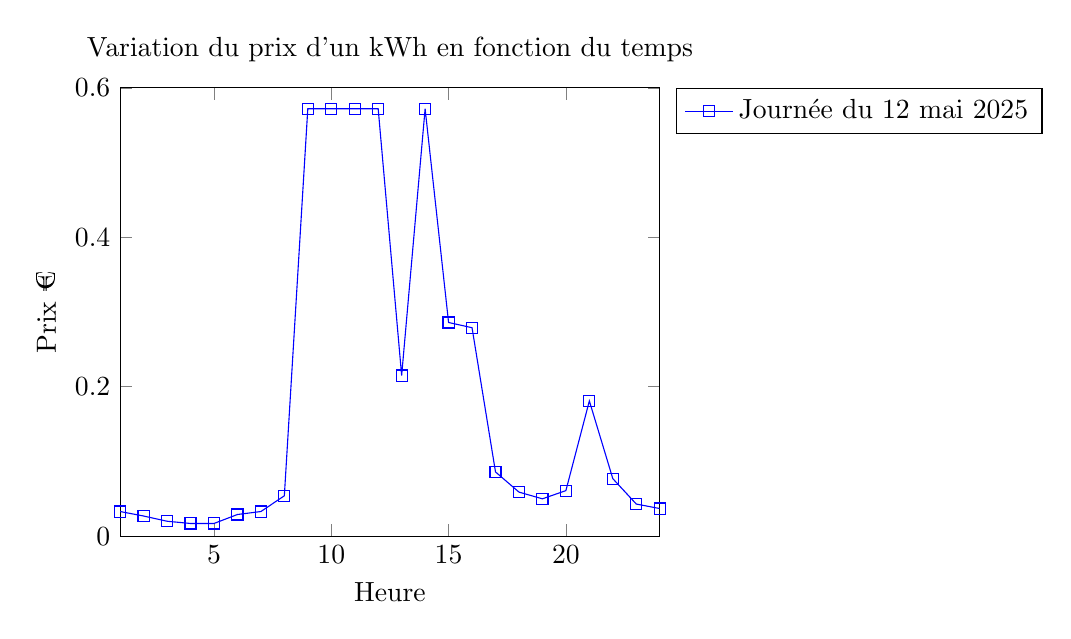
\begin{tikzpicture}
  \begin{axis}[
    title={Variation du prix d'un kWh en fonction du temps},
    xlabel={Heure},
    ylabel={Prix €},
    xmin=1, xmax=24,
    ymin=0, ymax=0.600,
    legend pos=outer north east
  ]

  \addplot[
    color=blue,
    mark=square,
    ]
    coordinates {
      (1, 0.033)(2, 0.027)(3, 0.020)(4, 0.017)(5, 0.017)(6, 0.029)
      (7, 0.033)(8, 0.054)(9, 0.572)(10, 0.572)(11, 0.572)(12, 0.572)
      (13, 0.215)(14, 0.572)(15, 0.286)(16, 0.279)(17, 0.086)(18, 0.059)
      (19, 0.050)(20, 0.061)(21, 0.181)(22, 0.077)(23, 0.043)(24, 0.037)
    };
    \legend{Journée du 12 mai 2025}

  \end{axis}
\end{tikzpicture}

Ces chiffres nous présentent un futur possible grâce à la smart grid, mais n'est qu'une projection dans le futur proche.

On s'aperçoit que la plupart des actions quotidiennes ne sont pas si différentes qu'en 2019, et que la plupart des
optimisations restent invisibles aux consommateurs.

La bourse en elle-même peut s'adapter à tous les niveaux de la smart grid. Le prix peut différer d'un quartier à un autre,
d'une ville à une autre mais est lissé du fait d'un environnement similaire et un échange entre les différents milieux micro.

\section{Risques et vecteur d'attaques}

% https://cyberguerre.numerama.com/624-peut-on-hacker-les-reseaux-electriques.html
L'informatique est le nouveau vecteur d'attaque du XXIème siècle, et le fait de le rendre primordial
dans un secteur clef tel que l'énergie ouvre de nouvelles portes aux pirates.

En effet, la smart city ajoute de nombreuses interfaces accessible pour tous qui sont toutes
vecteur d'attaque.


\begin{itemize}
  \item Le matériel qui est au centre de toutes les communications.
        Principal moyen de communication de la réalité, une altération de son
        comportement comporte le risque d'altérer les comportements logiciels.
  \item Les bases de données bien plus nombreuses peuvent être compromises.
        Ces données représentent la réalité et doivent restées aussi intègre que possible.
  \item Les logiciels utilisant ces données sont sensibles à différents vecteurs tels que le
        hameçonnage des comptes administrateurs et les failles logicielles.
  \item Les prises de décisions humaines peuvent être mises en péril avec de l'ingénierie sociale.
        Cela dans un but politique de la ville ou bien d'attaque terroriste.
\end{itemize}

Ces quatre facteurs déjà présents dans la ville d'aujourd'hui seront bien plus mises en avant avec
les réseaux intelligents.
